\documentclass[12pt]{article}
\usepackage[margin= 1in]{geometry} 
\usepackage{bibentry}
\usepackage{fourier}
\usepackage{ccaption}
\usepackage{stata}
\usepackage{amsmath}
\usepackage[pdftex]{graphicx}
\usepackage[colorlinks=true,
                      pdfstartview=FitV,
                      urlcolor=blue,
]{hyperref}

\usepackage{natbib}

\begin{document}

\thispagestyle{empty}%


\setlength{\parskip}{1ex plus 0.5ex minus 0.2ex}

\setcounter{secnumdepth}{-2}



\begin{flushleft}
Vanderbilt University\\Leadership, Policy and Organizations\\Class Number 9522\\ Spring 2018\\
\end{flushleft}

\begin{center}
\textbf{Diagnosing and Fixing Common Problems With Regression}
\end{center}

\section{Introduction}
\label{sec:introduction}

There are three ways to get a good intuitive grasp of whether there
might be some issues with your model fit:

\begin{enumerate}
\item Plot the data

\item Plot the data

\item Plot the data
\end{enumerate}


\section{Collinearity}
\label{sec:collinearity}

The test to use for collinearity in Stata is \texttt{vif}. The results
of the VIF (Variance Inflation Factor) test states whether inflation
has been increased because the covariate is correlated with the other
regressors. The rule of thumb with VIF's is that 10 is large, while 20
is unacceptable.

Stata's vif command can be run after a regression to check for
collinearity. 

\begin{stlog}
  
. 
. estat vif

    Variable |       VIF       1/VIF  
-------------+----------------------
          iq |     52.76    0.018955
       test3 |     52.24    0.019143
           s |      1.60    0.623911
         kww |      1.31    0.761735
         med |      1.18    0.848345
        expr |      1.15    0.867604
      tenure |      1.10    0.907839
         rns |      1.06    0.944157
        smsa |      1.05    0.948668
-------------+----------------------
    Mean VIF |     12.61

\end{stlog}

It looks like there's a big problem with the iq variable and the test3
variable. I first do an F test to see if they both belong in the
model. 

\begin{stlog}
  
. test test3 iq

 ( 1)  test3 = 0
 ( 2)  iq = 0

       F(  2,   748) =    6.65
            Prob > F =    0.0014

\end{stlog}

They are jointly significant, so I need to choose one to
eliminate. In this case I drop test3, re-run the model, and ask again
for variance inflation factors. 


\begin{stlog}
  
. local controls kww iq expr tenure rns smsa med 

. 
. reg `y' `x' `controls'

      Source |       SS       df       MS              Number of obs =     758
-------------+------------------------------           F(  8,   749) =   53.43
       Model |  50.6098566     8  6.32623207           Prob > F      =  0.0000
    Residual |  88.6762933   749  .118392915           R-squared     =  0.3634
-------------+------------------------------           Adj R-squared =  0.3566
       Total |   139.28615   757  .183997556           Root MSE      =  .34408

------------------------------------------------------------------------------
          lw |      Coef.   Std. Err.      t    P>|t|     [95% Conf. Interval]
-------------+----------------------------------------------------------------
           s |   .0878976   .0070921    12.39   0.000     .0739749    .1018203
         kww |   .0030669   .0019596     1.57   0.118    -.0007801    .0069139
          iq |   .0028559   .0011028     2.59   0.010      .000691    .0050208
        expr |   .0386396   .0063668     6.07   0.000     .0261407    .0511385
      tenure |   .0322462   .0078371     4.11   0.000     .0168608    .0476315
         rns |  -.0720075   .0289852    -2.48   0.013    -.1289095   -.0151055
        smsa |   .1302547   .0281144     4.63   0.000     .0750623    .1854471
         med |   .0055788    .004952     1.13   0.260    -.0041427    .0153004
       _cons |   3.840349   .1126832    34.08   0.000     3.619136    4.061561
------------------------------------------------------------------------------

. eststo full_model_a, title("Model 2:No Test 3")

. 
. estat vif

    Variable |       VIF       1/VIF  
-------------+----------------------
           s |      1.60    0.624254
          iq |      1.44    0.693400
         kww |      1.31    0.763785
         med |      1.18    0.848802
        expr |      1.15    0.870279
      tenure |      1.10    0.909065
         rns |      1.06    0.945150
        smsa |      1.05    0.949180
-------------+----------------------
    Mean VIF |      1.24

\end{stlog}

Much better! All vifs are now in an acceptable range. 

Remember that as a practical matter, collinearity does not bias your
estimates, it just makes them inefficient. It's usually just not that
serious a problem--- but it's worth checking to see if you're dealing
with an extreme case. 

\subsection{Quick Exercise}
\label{sec:quick-exercise}

What happens to VIFs when a variable of your choice is removed? 

\section{Heteroskedasticity}
\label{sec:heteroskedasticity}

Heteroskedasticity implies that the error terms are not identically
distributed, but instead may be related in some way to the regressors
or another factor. In this situation, our estimates are unbiased, but
our distributional assumptions about our \textit{variance} estimates
no longer hold, and standard tests of significance don't work. 

Figure \ref{fig:residplot1} shows the residuals for a regression of
log wages on various covariates plotted against years of
experience. This shows a highly heteroskedastic pattern in the
residuals. 

\begin{figure}[ht!]
  \centering
  \caption{Residuals Plotted Against Years of Experience}
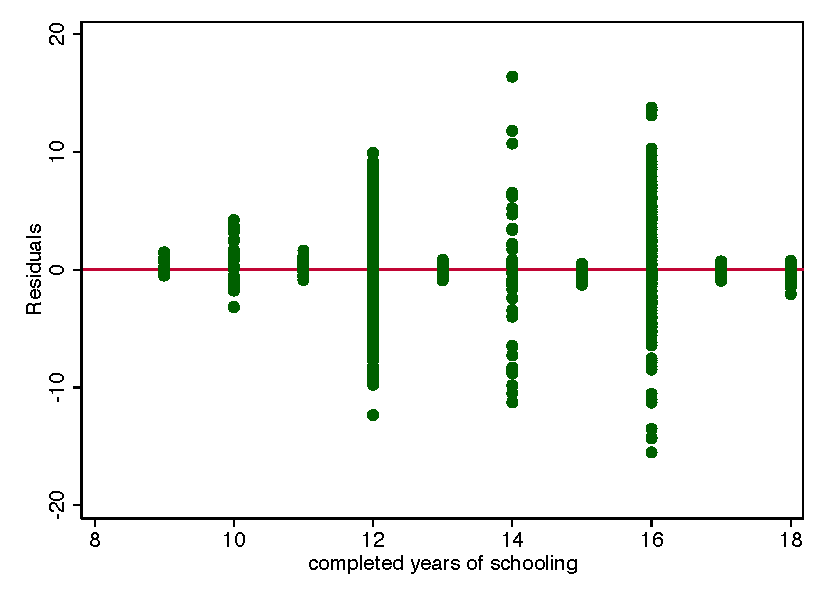
\includegraphics{het_results}
  \label{fig:residplot1}
\end{figure}

There are several ways of attempting to diagnose heteroskedastic
results. The Breusch-Pagan command as an omnibus test looks at whether
the variance of the squared residuals is related to any of the
regressors.We get this by regressing the square of the residuals on
the covariates and conducting an F test (or an LM test of the form
$nR^2$). If significant, then the covariates predict the residuals,
which indicatres a violation.  In Stata we get this result by using
the hettest command. Another option is the White test. The White test
follows the same basic form as the BP test, but instead uses the test
statistic $nR^2$ from the regression of the square of the residuals on
the covariates, their squares, and their cross-products. Like the BP
test, this test statistic has been shown to be distributed $\chi^2$
with degrees of freedom equal to the number of regressors in the
auxiliary regression.

\begin{stlog}
  
Breusch-Pagan / Cook-Weisberg test for heteroskedasticity 
         Ho: Constant variance
         Variables: fitted values of lw_het

         chi2(1)      =     4.69
         Prob > chi2  =   0.0304

. 
. estat hettest s expr

Breusch-Pagan / Cook-Weisberg test for heteroskedasticity 
         Ho: Constant variance
         Variables: s expr

         chi2(2)      =    21.50
         Prob > chi2  =   0.0000

. 
. /*White Test */
.   
. estat imtest, white

White's test for Ho: homoskedasticity
         against Ha: unrestricted heteroskedasticity

         chi2(42)     =     87.39
         Prob > chi2  =    0.0000

Cameron & Trivedi's decomposition of IM-test

---------------------------------------------------
              Source |       chi2     df      p
---------------------+-----------------------------
  Heteroskedasticity |      87.39     42    0.0000
            Skewness |       7.80      8    0.4534
            Kurtosis |      15.12      1    0.0001
---------------------+-----------------------------
               Total |     110.31     51    0.0000
---------------------------------------------------


\end{stlog}


In the first BP test above, the squared residuals are regressed on the
predicted values from the regression. In the second test, the squared
residuals are regressed on all of the covariates. And in the last,
the squared residuals are regressed on a specified subset of the
covariates. This last can help to identify the source of the non iid
error terms.  

You can correct for heteroskedasticity in a number of ways. The most straightforward
is to use robust standard errors, which take into account possible non
iid errors. If you suspect the errors in clusters (such as schools)
are correlated, you can calculated clustered standard errors, with
clustering at the group level. (N.B. My example below is artificial,
and honestly, incorrect).  

\begin{stlog}
  
. /*Robust s.e.'s*/
. reg lw_het `x' `controls', robust

Linear regression                                      Number of obs =     758
                                                       F(  8,   749) =    2.37
                                                       Prob > F      =  0.0158
                                                       R-squared     =  0.0202
                                                       Root MSE      =  3.9241

------------------------------------------------------------------------------
             |               Robust
      lw_het |      Coef.   Std. Err.      t    P>|t|     [95% Conf. Interval]
-------------+----------------------------------------------------------------
           s |   .2513847   .0746952     3.37   0.001     .1047479    .3980215
         kww |  -.0103424   .0237815    -0.43   0.664    -.0570288     .036344
          iq |  -.0189512     .01152    -1.65   0.100    -.0415666    .0036642
        expr |  -.0359087   .0682226    -0.53   0.599     -.169839    .0980215
      tenure |   .1580198   .0947811     1.67   0.096    -.0280485    .3440881
         rns |   .3126439   .3020458     1.04   0.301    -.2803131    .9056009
        smsa |   .3692457   .3106519     1.19   0.235    -.2406063    .9790977
         med |   -.028291   .0568756    -0.50   0.619    -.1399456    .0833635
       _cons |   4.345555   1.177585     3.69   0.000     2.033796    6.657315
------------------------------------------------------------------------------

. eststo full_model_robust, title("Model 2: Robust SE")

. 
. /*Clustered se.'s*/
. reg `y' `x' `controls', cluster(med)

Linear regression                                      Number of obs =     758
                                                       F(  8,    18) =  126.22
                                                       Prob > F      =  0.0000
                                                       R-squared     =  0.3634
                                                       Root MSE      =  .34408

                                   (Std. Err. adjusted for 19 clusters in med)
------------------------------------------------------------------------------
             |               Robust
          lw |      Coef.   Std. Err.      t    P>|t|     [95% Conf. Interval]
-------------+----------------------------------------------------------------
           s |   .0878976   .0090694     9.69   0.000     .0688436    .1069516
         kww |   .0030669   .0017164     1.79   0.091    -.0005391    .0066729
          iq |   .0028559   .0008181     3.49   0.003      .001137    .0045747
        expr |   .0386396   .0068981     5.60   0.000     .0241472     .053132
      tenure |   .0322462   .0049196     6.55   0.000     .0219105    .0425818
         rns |  -.0720075   .0236252    -3.05   0.007    -.1216422   -.0223729
        smsa |   .1302547    .014499     8.98   0.000     .0997935    .1607159
         med |   .0055788    .003547     1.57   0.133    -.0018732    .0130309
       _cons |   3.840349   .1197726    32.06   0.000     3.588716    4.091982
------------------------------------------------------------------------------

. eststo full_model_cluster, title("Model 2: Cluster SE")

. 
\end{stlog}

Angrist and Pischke suggest that we should assume that there IS
heteroskedasticity in the residuals, unless we can specifically prove
that there's none. Basically, you should always use robust standard
errors (or other appropriate variance estimation technique). 

\subsection{Quick Exercise}

Is there heteroskedasticity when we don't use the (made up) log wage
variable, but rather the real one?

\section{Data Scaling}
\label{sec:data-scaling}

The results of regression are invariant to linear transforms, but
sensitive to non-linear transforms. Changing the latter changes the
functional form of the regression model.

Results can be scaled in any number of ways. The most common is
standardized coefficients, which scales each coefficient as follows:

\begin{equation*}
  \hat{\beta_j^s}=\hat{\beta_j}\frac{SD(x_j)}{SD(y)}
\end{equation*}

In the results below I show the standardized coefficients for the
independent variables in the model, then transform the years of
schooling variable and re-run the model. While the coefficient
estimates change, the t-statistic and standardized coefficient does
not. 

\begin{stlog}
  .   
. /*Data Scaling*/
. 
. reg `y' `x' `controls'

      Source |       SS       df       MS              Number of obs =     758
-------------+------------------------------           F(  8,   749) =   53.43
       Model |  50.6098566     8  6.32623207           Prob > F      =  0.0000
    Residual |  88.6762933   749  .118392915           R-squared     =  0.3634
-------------+------------------------------           Adj R-squared =  0.3566
       Total |   139.28615   757  .183997556           Root MSE      =  .34408

------------------------------------------------------------------------------
          lw |      Coef.   Std. Err.      t    P>|t|     [95% Conf. Interval]
-------------+----------------------------------------------------------------
           s |   .0878976   .0070921    12.39   0.000     .0739749    .1018203
         kww |   .0030669   .0019596     1.57   0.118    -.0007801    .0069139
          iq |   .0028559   .0011028     2.59   0.010      .000691    .0050208
        expr |   .0386396   .0063668     6.07   0.000     .0261407    .0511385
      tenure |   .0322462   .0078371     4.11   0.000     .0168608    .0476315
         rns |  -.0720075   .0289852    -2.48   0.013    -.1289095   -.0151055
        smsa |   .1302547   .0281144     4.63   0.000     .0750623    .1854471
         med |   .0055788    .004952     1.13   0.260    -.0041427    .0153004
       _cons |   3.840349   .1126832    34.08   0.000     3.619136    4.061561
------------------------------------------------------------------------------

.   
. reg `y' `x' `controls', beta

      Source |       SS       df       MS              Number of obs =     758
-------------+------------------------------           F(  8,   749) =   53.43
       Model |  50.6098566     8  6.32623207           Prob > F      =  0.0000
    Residual |  88.6762933   749  .118392915           R-squared     =  0.3634
-------------+------------------------------           Adj R-squared =  0.3566
       Total |   139.28615   757  .183997556           Root MSE      =  .34408

------------------------------------------------------------------------------
          lw |      Coef.   Std. Err.      t    P>|t|                     Beta
-------------+----------------------------------------------------------------
           s |   .0878976   .0070921    12.39   0.000                 .4573323
         kww |   .0030669   .0019596     1.57   0.118                 .0522099
          iq |   .0028559   .0011028     2.59   0.010                 .0906704
        expr |   .0386396   .0063668     6.07   0.000                 .1896665
      tenure |   .0322462   .0078371     4.11   0.000                 .1258147
         rns |  -.0720075   .0289852    -2.48   0.013                -.0745005
        smsa |   .1302547   .0281144     4.63   0.000                 .1386435
         med |   .0055788    .004952     1.13   0.260                 .0356506
       _cons |   3.840349   .1126832    34.08   0.000                        .
------------------------------------------------------------------------------

. eststo full_model_beta, title("Model 2: Standardized Coefficients")

. 
. gen expr_new=1+2*s

. 
. local x expr_new

. 
. reg `y' `x' `controls', beta

      Source |       SS       df       MS              Number of obs =     758
-------------+------------------------------           F(  8,   749) =   53.43
       Model |  50.6098566     8  6.32623207           Prob > F      =  0.0000
    Residual |  88.6762933   749  .118392915           R-squared     =  0.3634
-------------+------------------------------           Adj R-squared =  0.3566
       Total |   139.28615   757  .183997556           Root MSE      =  .34408

------------------------------------------------------------------------------
          lw |      Coef.   Std. Err.      t    P>|t|                     Beta
-------------+----------------------------------------------------------------
    expr_new |   .0439488    .003546    12.39   0.000                 .4573323
         kww |   .0030669   .0019596     1.57   0.118                 .0522099
          iq |   .0028559   .0011028     2.59   0.010                 .0906704
        expr |   .0386396   .0063668     6.07   0.000                 .1896665
      tenure |   .0322462   .0078371     4.11   0.000                 .1258147
         rns |  -.0720075   .0289852    -2.48   0.013                -.0745005
        smsa |   .1302547   .0281144     4.63   0.000                 .1386435
         med |   .0055788    .004952     1.13   0.260                 .0356506
       _cons |     3.7964   .1134835    33.45   0.000                        .
------------------------------------------------------------------------------

\end{stlog}

Rescaling on Z scores can make sense in many applications, but it is
not a way to compare coefficients. 

\subsection{Quick Exercise}

Rescale the parental education variable using both a linear and a
non-linear transform and check to see what
difference it makes in the results. 

\section{Functional Form}
\label{sec:functional-form}

In checking on functional form, your best bet is almost always using
graphical approaches. Below I plot the wages as a function of years of
schooling, then plot the a line based on local linear regression. 

\begin{figure}[ht!]
  \centering
  \caption{Wages as a function of schooling}
  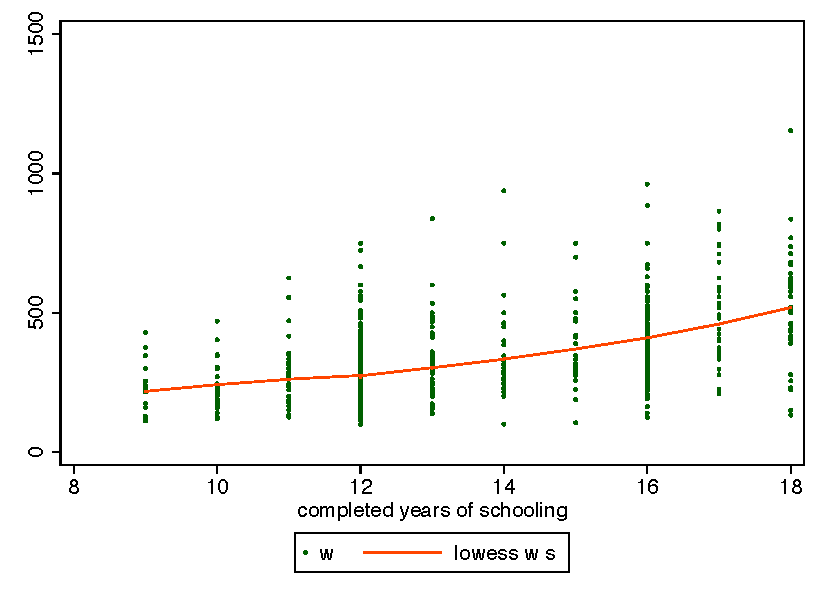
\includegraphics{lowess1}
  \label{fig:lowess1}
\end{figure}

Next I plot both a lowess line and a linear fit to see what the
results of a simple regression might look like. 

\begin{figure}[ht!]
  \centering
  \caption{Wages as a function of schooling, linear fit to data}
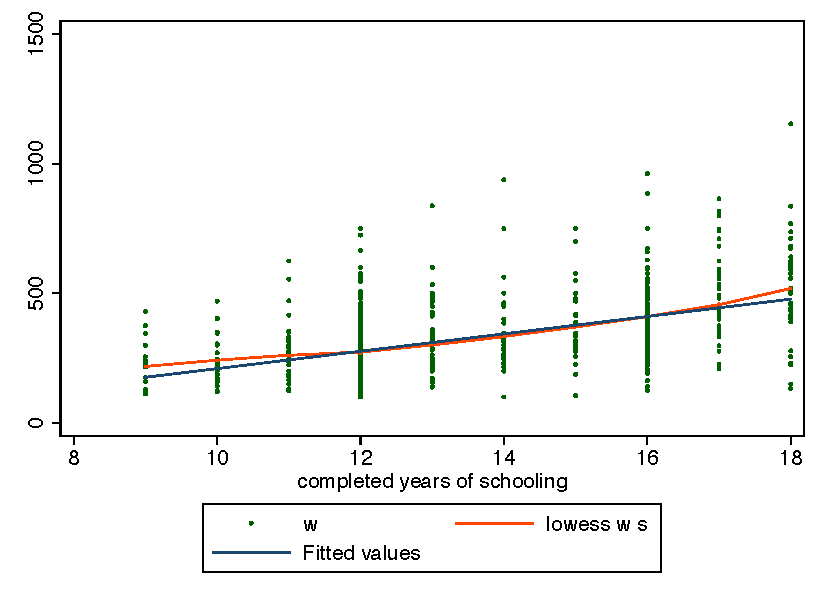
\includegraphics{lfit1}
  \label{fig:lfit}
\end{figure}


\begin{figure}[ht!]
  \centering
  \caption{Wages as a function of schooling, multiple functional forms}
  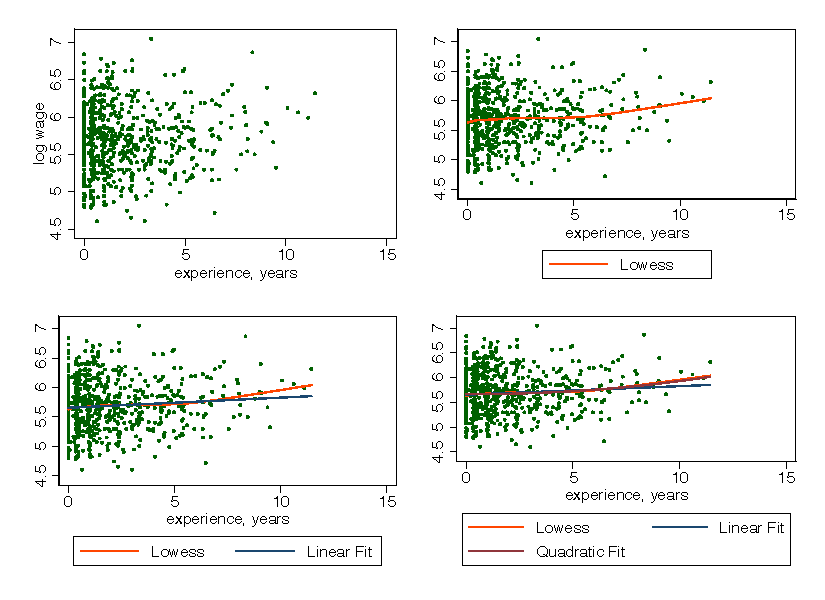
\includegraphics{logfit}
  \label{fig:mutlfit}
\end{figure}
\subsection{Quick Exercise}
Using a similar approach to the one I use in the do file, check on the
functional form of the relationship between wages and kww scores. 

\subsection{The log transformation}
\label{sec:log-transformation}

We covered this previously. Remember that the log transformation is a
good idea when the dependent variable is on some kind of exponential
scale. 

\section{Influential Observations}
\label{sec:infl-observ}

Regression is quite sensitive to outliers. A data point can ``pull''
the regression line quite far away given its distance from that
line. We test for influential measures using several different
measures including 
leverage, dfits, cooks D, or dfbeta.

\begin{itemize}
\item Leverage is measured in the scale of the dv and is the basic
  measure of influence from a residual.

\item The dfits statistic compares the standardized residual for every
  observation on the scale of the standard error of the regression. 

\item Cook's d combines information regarding leverage---how
  influential the observation is on the results--- and the size of the
  residual---how far off the prediction the actual result is. 

\item Dfbetas are calculated for every unit AND every coefficient, and
  state how far the coefficient would move should that case be
  excluded. 

\end{itemize}

A leverage plot is a good place to being examining the data for
influential observations.

\begin{figure}[ht!]
  \centering
  \caption{Leverage Plot}  
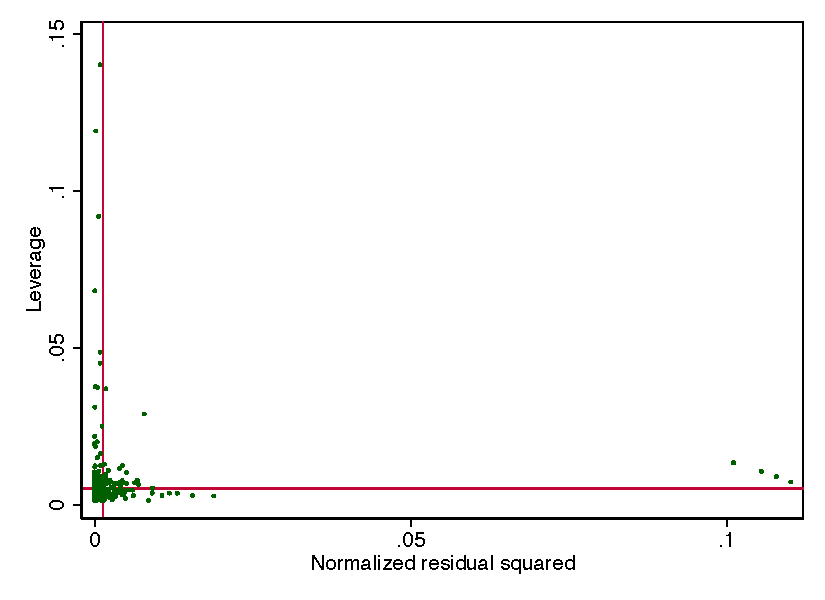
\includegraphics{levplot}
  \label{fig:levplot}
\end{figure}

The leverage plot shows the leverage of each observation on the y axis
and the square of the residual on the x axis. The red lines on each
axis are the cutoff points for ``large'' leverage or residual stats. 

For each of the measures leverage, dfits, cooks' D and dfbeta, the
procedure is the same. Calculate the measure, then look for
observations that exceed a given rule of thumb. Here's that procedure
applied to leverage. 

For DFits, the measure is given by:

\begin{equation*}
  DFITS_j=r_j\sqrt{frace{h_j}{1-h_j}}
\end{equation*}

Where $r_j$ is a studentized residual:

\begin{equation*}
  r_j=\frac{\epsilon_j}{s_{(j)}}\sqrt{1-h_j}
\end{equation*}

The rule of thumb cutoff for dfits is $|{DFITS_j}|>2 \sqrt{k/N}$.

For Cook's D, the calculation is:

\begin{equation*}
  D_i=\frac{\sum_{i=1}^n(\hat{y}_i-\hat{y}_{i(w)})^2}{p MSE}
\end{equation*}

Where $\hat{y}_i$ is the prediction with observation $i$ and
$\hat{y}_{i(w)}$ is the prediction \emph{without} observation $i$. 

The rule of thumb for cooks D is to investigate values over $4/n$. 

Last, the calculation for DFBETA is given by: 

\begin{equation*}
  DFBETA_j=\frac{r_jv_j}{\sqrt{v^2(1-h_j}}
\end{equation*}

This tells you how much a regression coefficient would change if unit
$j$ was excluded. The cutoff suggested for DFBETA is $2/\sqrt{n}$. 

\begin{stlog}
. /* Leverage and outliers  */
.   
. predict lev if e(sample), leverage

. 
. predict resid if e(sample), resid

. 
. gen  resid2=resid^2

. 
. gsort -lev

. 
. list w_influence s lev resid2 in 1/10

     +-------------------------------------+
     | w_infl~e    s        lev     resid2 |
     |-------------------------------------|
  1. | 555.0176   11   .1402453   16845.92 |
  2. | 401.0154   12   .1191845   3480.702 |
  3. | 430.0924    9   .0920351   12456.28 |
  4. | 454.8647   12   .0682902    395.947 |
  5. | 204.9979   10   .0488069   16943.56 |
     |-------------------------------------|
  6. | 288.0114   12    .045244   17041.28 |
  7. | 367.9695   12    .037804   1923.356 |
  8. | 375.0278    9   .0375033   8861.435 |
  9. | 600.0421   12   .0371506   35667.26 |
 10. | 332.9526   11   .0312744   839.5032 |
     +-------------------------------------+
\end{stlog}

\subsection{Quick Exercise}

Run the same regression without the schooling variable. Check for
outliers using both graphical and tabular methods. 


\end{document}


%%% Local Variables: 
%%% mode: latex
%%% TeX-master: t
%%% End: 
